\documentclass[unicode, notheorems, aspectratio=169]{beamer}
% Aspect ratio: https://tex.stackexchange.com/questions/14336/latex-beamer-presentation-package-169-aspect-ratio#answer-14339
\usepackage{etex}  % Should be second line. Otherwise tikz raises error.
\hypersetup{pdfpagemode=FullScreen}

% If you have more than three sections or more than three subsections in at least one section,
% you might want to use the [compress] switch. In this case, only the current (sub-) section
% is displayed in the header and not the full overview.
\mode<presentation>
{
  \usetheme{Madrid}
  \usecolortheme{seahorse}
}

% https://tex.stackexchange.com/questions/106789/why-does-usepackaget2afontenc-take-over
\usepackage[T2A,T1]{fontenc}
\usepackage[english]{babel}
\usepackage{amsthm}
\usepackage[noend]{algorithmic}
\usepackage{algorithm}
\usepackage[all]{xy} % for graph plotting
% \usepackage{times}
\usepackage{tikz}
\usetikzlibrary{arrows,shapes,backgrounds}
\usepackage{textcomp} % euro sign
\usepackage[official]{eurosym}
\usepackage{ulem} % strike
\usepackage{color} % use colors (in minted)

% tables
\usepackage{booktabs}
\usepackage{multirow}

%% Code highlight
% Doc: http://ftp.yzu.edu.tw/CTAN/macros/latex/contrib/listings/listings.pdf
\usepackage{listings}
\usepackage{minted}
\definecolor{LightGray}{rgb}{0.95,0.95,0.95}
\setminted{bgcolor=LightGray}
%\usemintedstyle{monokai}
% ftp://ftp.dante.de/tex-archive/macros/latex/contrib/minted/minted.pdf
% Note: to use minted, install pygments http://pygments.org/ and add "-shell-escape" flag to latex command.
% Minted doc: http://ftp.yzu.edu.tw/CTAN/macros/latex/contrib/minted/minted.pdf
%% END: Code highlight

\usepackage{helvet}

\title[JSON-RPC standard and library]{Reinvent the wheel and build the most popular JSON-RPC library}
\author[Kirill Pavlov <k@p99.io>]{Kirill Pavlov, \small{@pavlov99}}
\institute[]{Technical Recruiter, Terminal 1}
\titlegraphic{
\includegraphics[width=3cm]{./images/pycon-logo}}
\date{14:30 -- 15:00, November 4, 2017}

\definecolor{t1_light}{RGB}{38,47,112}
\definecolor{t1_dark}{RGB}{39,47,56}
\definecolor{t1_blue}{RGB}{50,121,235}

\setbeamertemplate{title page}[default][colsep=-4bp,rounded=true]
\setbeamertemplate{itemize items}[default]
\setbeamertemplate{enumerate items}[default]

\setbeamercolor*{palette primary}{use=structure,fg=white,bg=t1_light}
\setbeamercolor*{palette secondary}{use=structure,fg=white,bg=t1_dark}
\setbeamercolor*{palette tertiary}{use=structure,fg=white,bg=t1_blue}

\setbeamercolor{itemize item}{fg=t1_blue}
\setbeamercolor{itemize subitem}{fg=t1_blue}
\setbeamercolor{enumerate item}{fg=t1_dark}
\setbeamercolor{enumerate subitem}{fg=t1_dark}

\setbeamertemplate{section in toc}{%
  {\color{t1_dark}\inserttocsectionnumber.}~\inserttocsection}
\setbeamercolor{subsection in toc}{bg=white,fg=structure}
\setbeamertemplate{subsection in toc}{%
  \hspace{1.2em}{\color{t1_dark}\rule[0.3ex]{3pt}{3pt}}~\inserttocsubsection\par}
  
% Set beamer blocks
\setbeamertemplate{blocks}[rounded][shadow=false]
\addtobeamertemplate{block begin}{\pgfsetfillopacity{0.8}}{\pgfsetfillopacity{1}}

\setbeamercolor*{block title example}{fg=white,bg= t1_light}
\setbeamercolor*{block body example}{fg=white,bg= t1_dark}

% remove page navigation.
\beamertemplatenavigationsymbolsempty

% Set link colours
\definecolor{links}{HTML}{2A1B81}
\hypersetup{colorlinks,linkcolor=,urlcolor=links}

\begin{document}
% For every picture that defines or uses external nodes, you'll have to
% apply the 'remember picture' style. To avoid some typing, we'll apply
% the style to all pictures.
\tikzstyle{every picture}+=[remember picture]

% By default all math in TikZ nodes are set in inline mode. Change this to
% displaystyle so that we don't get small fractions.
\everymath{\displaystyle}

% This presentation shows ability of spark to work with data.
% It covers data processing, pipelining, feature engineering and algorithms available in Spark.

\begin{frame}
\titlepage
\end{frame}

\begin{frame}{Journey started 4+ years ago Sep 30, 2013}
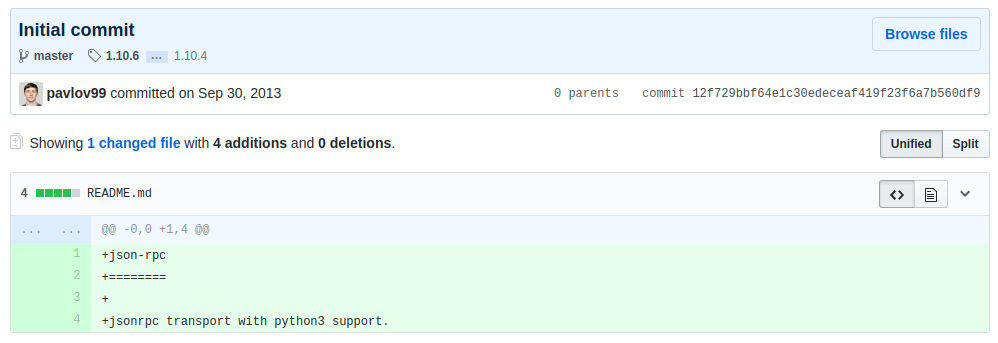
\includegraphics[width=.95\paperwidth]{./images/json-rpc-initial-commit}
\end{frame}

\begin{frame}{Table of content}
	% \tableofcontents[currentsection]
    \tableofcontents
\end{frame}

\section{What is JSON-RPC}
\begin{frame}{Table of content}
	\tableofcontents[currentsection]
\end{frame}

\begin{frame}{JSON-RPC 101}
\begin{center}
\Huge ``It is a very simple protocol\footnotemark''
\\[5pt]
\rightline{{\rm --- Wikipedia}}
\end{center}

\vfill
\begin{center}
JSON-RPC = \href{https://en.wikipedia.org/wiki/JSON}{JavaScript Object Notation} + \href{https://en.wikipedia.org/wiki/Remote\_procedure\_call}{Remote Procedure Call}.
\end{center}

\footnotetext[1]{
Wikipedia article \href{https://en.wikipedia.org/wiki/JSON-RPC}{https://en.wikipedia.org/wiki/JSON-RPC}}
\end{frame}

\begin{frame}{A brief history of JSON-RPC}
\begin{itemize}
\item 1998 \href{https://en.wikipedia.org/wiki/XML-RPC}{XML-RPC}
\item 2000 \href{https://en.wikipedia.org/wiki/Representational\_state\_transfer}{REST} specification
\item 2005 \href{https://en.wikipedia.org/wiki/JSON-RPC}{JSON-RPC 1.0}
\item 2007 \href{http://json-rpc.org/} {JSON-RPC 1.1} http://json-rpc.org/
\item 2010 \href{http://www.jsonrpc.org/specification}{JSON-RPC 2.0} http://www.jsonrpc.org/specification
\item 2010 Django REST Framework
\item 2017 This PyCon!
\end{itemize}
\end{frame}

\begin{frame}[fragile]{JSON-RPC 2.0 Spec in 1 minute}
\begin{enumerate}
\item Request:
\begin{minted}{javascript}
{"jsonrpc": "2.0", "method": METHOD, "params": PARAMS, "id": ID}
\end{minted}
\item Notification -- Request without `id`, does not receive a response
\item Batch support
\item Response:
\begin{minted}{javascript}
{"jsonrpc": "2.0", "result": RESULT, "id": ID}
\end{minted}
\item Error:
\begin{minted}{javascript}
{
  "jsonrpc": "2.0",
  "error": {
    "code": INT, "message": MESSAGE, "data": DATA
  },
  "id": ID
}
\end{minted}
\end{enumerate}
\end{frame}

\begin{frame}[fragile]{JSON-RPC 2.0 Example 1: success}
1. Positional parameters:
{\small
\begin{minted}{javascript}
--> {"jsonrpc": "2.0", "method": "sub", "params": [42, 23], "id": 1}
<-- {"jsonrpc": "2.0", "result": 19, "id": 1}
\end{minted}
}
\vfill
2. Named parameters:
{\small
\begin{minted}{javascript}
--> {"jsonrpc": "2.0", "method": "sub", "params": {"b": 23, "a": 42}, "id": 2}
<-- {"jsonrpc": "2.0", "result": 19, "id": 2}
\end{minted}
}
\vfill
3. Notification:
{\small
\begin{minted}{javascript}
--> {"jsonrpc": "2.0", "method": "foobar"}
\end{minted}
}
\end{frame}

\begin{frame}[fragile]{JSON-RPC 2.0 Example 2: error}
4. Invalid JSON:
{\small
\begin{minted}{javascript}
--> {"jsonrpc": "2.0", "method": "foobar, "params": "bar", "baz]
<-- {... "error": {"code": -32700, "message": "Parse error"}, "id": null}
\end{minted}
}
\vfill
5. Method does not exist:
{\small
\begin{minted}{javascript}
--> {"jsonrpc": "2.0", "method": "foobar", "id": "1"}
<-- {... "error": {"code": -32601, "message": "Method not found"}, "id": "1"}
\end{minted}
}
\vfill
6. Invalid request:
{\small
\begin{minted}{javascript}
--> {"jsonrpc": "2.0", "method": 1, "params": "bar"}
<-- {... "error": {"code": -32600, "message": "Invalid Request"}, "id": null}
\end{minted}
}
\end{frame}

\begin{frame}[fragile]{JSON-RPC 2.0 Example 3: batch}

{\small
\begin{minted}{javascript}
--> [
      {"jsonrpc": "2.0", "method": "sum", "params": [1,2,4], "id": "1"},
      {"jsonrpc": "2.0", "method": "notifyHello", "params": [7]},
      {"jsonrpc": "2.0", "method": "subtract", "params": [42,23], "id": "2"},
      {"foo": "boo"},
      {"jsonrpc": "2.0", "method": "getData", "id": "9"} 
    ]
<-- [
      {"jsonrpc": "2.0", "result": 7, "id": "1"},
      {"jsonrpc": "2.0", "result": 19, "id": "2"},
      {"jsonrpc": "2.0", "error": {"code": -32600, "message": "Invalid Request"},
        "id": null},
      {"jsonrpc": "2.0", "result": ["hello", 5], "id": "9"}
    ]
\end{minted}
}
\end{frame}


\section{Reasons behind "json-rpc" library and why re-invent the wheel}
\begin{frame}{Table of content}
	\tableofcontents[currentsection]
\end{frame}

\begin{frame}{Background}
\begin{itemize}
\item Multichannel, 2012-2013. A lot ($\sim$10) of micro services. 3 FTE to support.
\item HTTP and AMQP (RabbitMQ) protocols.
\item API is simple, reliable and easy to understand (has specification). REST is not strict.
\item Fast to write servers and clients. Note: error handling takes 40\%-60\% of time.
\end{itemize}
\end{frame}


\begin{frame}{Think REST is simple?}
\begin{itemize}
\item Could one create an object with PUT?
\item Should one partially update with PUT or PATCH?
\item How many HTTP response codes do you remember? 201/202/403/409/418\footnotemark
\item Should /resource/<id> return an object or list with one object?
\item How to send a meta-information? E.g. total number of objects in pagination?
\end{itemize}

\footnotetext[2]{201 Created, 202 Accepted, 403 Forbidden, 409 Conflict, 418 I'm a teapot}
\end{frame}

\begin{frame}{Alternative implementations}
\begin{center}
	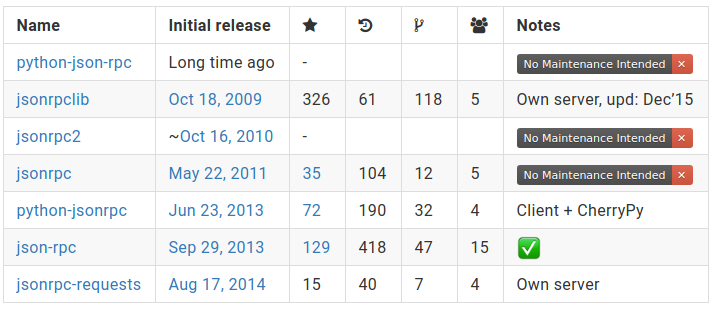
\includegraphics[width=.95\paperwidth]{./images/alternatives} 
\end{center}

{\small
Didn't have a good library pluggable to any backend. Alternatives had own http/queue servers.
}
\end{frame}

\begin{frame}{json-rpc feature summary}
\begin{itemize}
\item Super portable. Solve one thing and solve it good. Supports all practical pythons.
\item Implements 100\% of standard (1.0 and 2.0). There is no reason to write another lib.
\item 220+ test cases. In the beginning I thought would be ~30. Lesson: implementation is not as easy even for simple json-rpc.
\item Optional Django and Flask backends. No dependencies required.
\end{itemize}

Result: "most popular" json-rpc library. Was used in Ansible 1.0!
\end{frame}

\section{Demo: Vanilla and Django API servers}
\begin{frame}
\begin{center}
		{\huge Demo Time}
		
		\vspace{5mm}
		Vanilla and Django API severs \\
		\href{https://github.com/pavlov99/presentations/tree/master/2017-11-04-pycon}{https://github.com/pavlov99/presentations/tree/master/2017-11-04-pycon}
	\end{center}
\end{frame}

\section{How to make a good library}
\begin{frame}{Table of content}
	\tableofcontents[currentsection]
\end{frame}

\begin{frame}{Checklist}
\begin{enumerate}
\item 90\% of functionality takes 10\% of time. The other 10\% takes all of your time.
\item Make something people want.
\item Must have: documentation (README), CI, green tests, quickstart and examples.
\item Create a community: Code of Conduct, Contributors, License, Issue/Pull request templates.
\item Low barier for testing, contribution and new release.
\end{enumerate}
\end{frame}

\begin{frame}
\begin{center}
	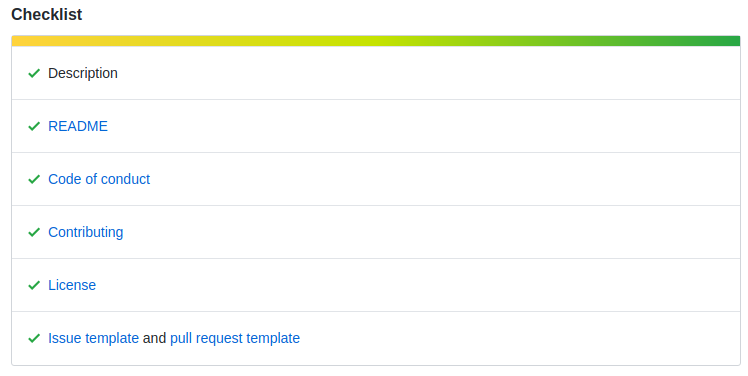
\includegraphics[width=.95\paperwidth]{./images/community-profile} 
\end{center}
\end{frame}

\begin{frame}{Promotion}
\begin{itemize}
\item Choose a good name and desctiption. Be an SEO expert!
\item Link from "standard description" website and/or \href{https://web.archive.org/web/20160624152815/https://en.wikipedia.org/wiki/JSON-RPC}{Wikipedia} [24-06-2016].
\item Bitcoin communities and crypto currencies exchanges, e.g. \href{https://counterparty.io/}{counterparty.io}.
\item StackOverflow \href{https://stackoverflow.com/questions/5467919/json-rpc-python-client/19887957\#19887957}{questions}.
\item Code of Conduct (Contributor Convenant) adopters via Pull Requests.
\end{itemize}
\end{frame}

\begin{frame}{What drives me to contribute}
\begin{center}
	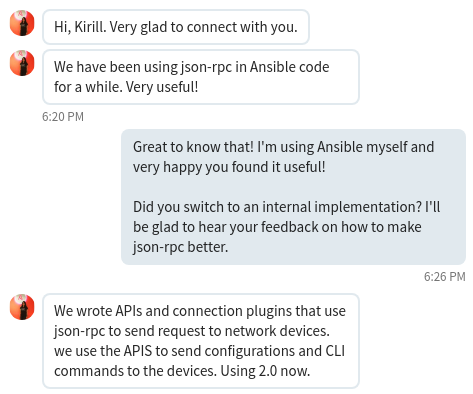
\includegraphics[height=.8\textheight]{./images/ansible}\qquad
	
\includegraphics[height=.8\textheight]{./images/drives-to-contribute}
\end{center}
\end{frame}

\begin{frame}
\begin{center}
{\huge Thank you!}

\vfill
Kirill Pavlov <k@p99.io>, Recruiter, \href{https://t1.gl/k}{Terminal 1}.

{\small
GitHub: \href{https://github.com/pavlov99}{@pavlov99} |
Presentation: \href{https://github.com/pavlov99/presentations/tree/master/2017-11-04-pycon}{2017-11-04-pycon} |
\href{https://github.com/pavlov99/json-rpc}{json-rpc} \\
\#jobs \href{https://t1.gl/k}{https://t1.gl/k} \\
"Python \& AWK" talk tomorrow 14:40-15:10
}
\end{center}
\end{frame}

\end{document}
